\chapter{序論}

\section{研究背景}

高齢者施設は,現代社会の基盤となるシステムである.一方で,少子高齢化やそれに伴う介護士の不足は,医療サービス利用者にとって大きな問題である.これらの問題を解決するために,介護士の労働環境の改善や医療施設の拡充等が検討されている.医療現場は,一旦変更してしまうと容易に元に戻すことが難しい.しかも医療現場は非常に複雑であり,サービスの被提供者のプライベートや安全と密接に関連していることから,実験を行うこと自体が時間・コスト・安全の面から現実的ではない.このため,最新技術の導入等の実験を行い,それらの効果検証が出来る医療シミュレータの開発が急を要しているものの,医療現場はプライベートな空間であり,これまで現実データを十分に獲得することが出来ず,有用なシミュレータの構築が難しかった.しかし,今後の日本における医療の重要性を考えると,個人の特性や意志を持った主体として介護者,被介護者を取り扱い,それらの詳細な相互作用を取り入れたシミュレータの構築が必要であると考えられる.

\subsection{日本の抱える諸課題}

我が国では,世界に先駆けて少子高齢化が深刻化している.1950年時点で5%に満たなかった高齢化率(65歳以上人口割合)は,1985年には10.3%,2005年には20.2%と急速に上昇し,2015年は26.7%と過去最高となっている.将来においても,2060年まで一貫して高齢化率は上昇していくことが見込まれており,2060年時点では約2.5人に1人が65歳以上の高齢者となる見込みである\cite{ex_kousei_v1}.
直近では,2025年問題が迫っている.2025年問題とは,1947年から1949年生まれのいわゆる団塊の世代が65歳以上になり、高齢化率がさらに上昇するという問題のことである\cite{2025_problem}.
このような少子高齢化に伴い、様々な問題が引き起こされている.生産年齢人口の減少により、生産活動と消費活動の衰えが経済全体の停滞をもたらすことはもちろん、社会保障費の増大による国家財政の不安定化も免れない.
生産年齢人口の現象が引き起こす経済の衰退は図\ref{population_GDP_relation}のように如実に現れている.

\begin{figure}[htb]
 \begin{center}
 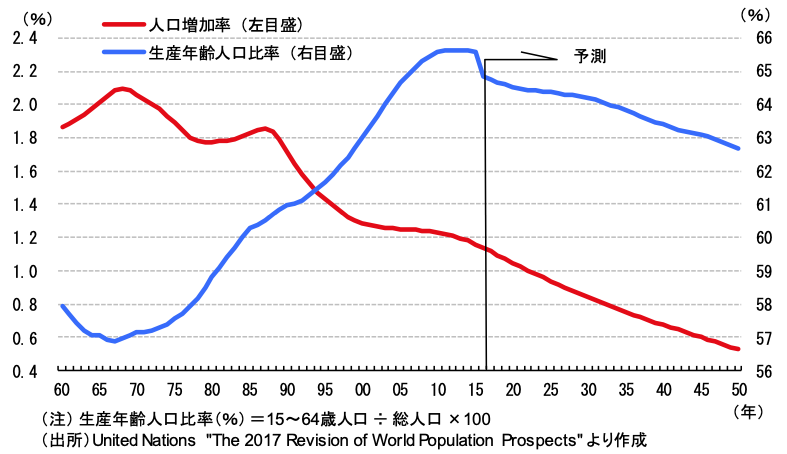
\includegraphics[scale=0.6]{figures/population_GDP_relation}
 \caption[経済衰退]{経済衰退 \label{population_GDP_relation}}
 \end{center}
\end{figure}

また、社会保障費の増大も深刻であり、2025年度には対GDP比で24.4%になるとされている\cite{social_security}.

\subsection{医療現場のマクロ課題}

一方で,長期の医療,介護が必要となる高齢者へサービスを提供している施設とその従業員は多大な問題を抱えている.
第一に,介護を必要とする高齢者向け施設が不足している.「特別養護老人ホーム」「介護老人保健施設」「介護療養型医療施設」の3類型の定員数(介護療養型医療施設は病床数)合計にしめる65歳以上人口割合は軒並み4%を切っており、十分な施設供給ができているとは言えない\cite{lack_facility_1}.
特に特別養護老人ホームの不足は深刻だ.2014年の厚生労働省の発表では,特別養護老人ホームの入所申込者数(いわゆる待機老人数)が2013年度に52.4万人と発表するなど、介護施設の不足が改めて確認された.特別養護老人ホームへの入所申込者数は、2009年度調査の42.1万人から約10万人増加している。特別養護老人ホームの数は2012年度時点でで全国で7,605施設、総定員数は50.7万人である.つまり2012年時点ですら,総定員数以上の入所希望者がおり、施設が不足していたことがわかる\cite{lack_facility_2}.
2018年に厚生労働省は,全国の市町村が策定した第7期の介護保険事業計画を踏まえた,必要介護者数を公表した.
それによれば、介護職員の需要は2020年度で216万494人、2025年度で244万6562人に増える.足下の2016年度の実績は189万8760人で、2025年度との差は54万7802人であり,毎年6万人の補充をし続けなければならない.
しかし、目先の介護士人数を増やしたところで,他にも大きな問題点が残留している.介護士の離職率の高さである.
常勤労働者の離職率を比較して見ると,産業全体の離職率11.6%であるのに対して介護職員の離職率は19.0%となっている.
この状況は,直近7年間で変動していない.平成22年度の産業全体の離職率は14.5%であるのに対し,介護職員の離職率は17.8%であって、産業全体の離職率を介護職員の離職率が下回ったことがない.

\subsection{高齢者施設運営における課題}
我が国では,平成12年に医療保険制度に加えて,「介護保険制度」が導入された.介護保険の総費用は,平成12年から平成21年にかけて,3.6兆円から7.4兆円へ年10%を超える伸びで増大し,月間利用者も184万人(平成12年度)から344万人(平成19年度)と増加した.当初218万人だった要介護認定者が,現在数倍になっており,要介護高齢者の状態像で,認知症・廃用症候群・脳卒中の3大症状の対策が重要であると言われている.
今村ら\cite{nursing_management}によると,今後の施設運営で考慮すべき問題点は大きく8点挙げられている.

\begin{itemize}
 \item 「昭和ヒトケタ世代」から「第一次ベビーブーマー」へ移行した際の問題
 \item 認知症の増加の問題
 \item 単独世帯の増加の問題
 \item 都市部の高齢化の問題
 \item 看取り(死亡)の場所と体制の問題
 \item 介護のリハビリテーションの問題
 \item 医療と介護の連携の問題
 \item 介護従事者の確保の問題
\end{itemize}

以上のように,今後高齢者施設を適切に運営していくためには,すぐれた療養環境の提供と個別ケアが求めらていると言える.また,施設だけで完結するのではなく,地域や家族の協力のもと,適切な在宅ケアを提供していく必要がある.

\subsection{国の取り組み}

前述の通り, 厚生労働省は毎年6万人の介護職員増員を目標としている.増員施策として大きく「参入促進」「労働環境・処遇の改善」を行っている\cite{nurse_solution}.
参入促進に関して、地域住民や学校の生徒に対する介護や介護の仕事の理解促進や若者・女性・高齢者など多様な世代を対象とした介護の職場体験といった施策は従来から行われていた.
それに加えて,三つの新たな施策が行われている.
まず,介護に関する入門的研修の実施からマッチングまでの一体的支援事業の創設である.介護未経験者の介護分野への参入のきっかけを作るとともに,参入障壁となっている介護に関する様々な不安を払拭するため,介護業務の入門的な知識・技術の修得のための研修を導入し,介護人材のすそ野を拡げ,中高年齢者など多様な人材の参入を促進するという施策である.
次に,将来の介護サービスを支える若年世代の参入促進事業である.介護に関する教育機関である介護福祉士養成施設において,将来の介護現場を担う世代に対する介護の専門性や意義を伝達する取組や,今後増加することが予想される留学生への日本語学習支援等による質の高い人材の養成・確保に係る取組を推進している.
加えて,介護福祉士国家資格の取得を目指す外国人留学生の受入環境整備事業の創設も行っている.介護施設等による外国人留学生への奨学金等の支給と介護福祉士資格の取得を目指す留学生と受入介護施設等とのマッチング支援によって,外国人の介護士の活用を始めた.
また,労働環境・処遇の改善について,管理者へ雇用改善方策の普及を主に行っている.具体的には,管理者に対する雇用管理改善のための労働関係法規,休暇・休職制度等の理解のための説明会の開催などが行われている.
こうした施策によって介護士の母数そのものを増やすことも重要であるが,介護士1人当たりが対応できる要介護者を増やすことも同程度に必要なことである.
その実現可能性を高めるものとして,医療技術の発達は目覚ましい.

\subsection{医療技術の発達}

医療技術の一例として,医療ロボットとハイテク福祉機器について言及したい. 厚生労働省は,2040年を展望した中長期ビジョンである「未来イノベーション WG 」の取りまとめを踏まえた医療福祉分野における取組を検討し,2019年度中に具体化することを目標としており,医療・介護現場のハイテク化に努めている.\cite{care_robots}
第一に,介護ロボットとは,情報を感知し,判断し,動作するという3要素を有する知能化した機械システムのことである.具体的には,図\ref{care_robots}のように,要介護者の移乗支援を行う装着型パワーアシストや,要介護者の排泄支援を行う自動排泄処理装置などが該当する.

\begin{figure}[htb]
 \begin{center}
 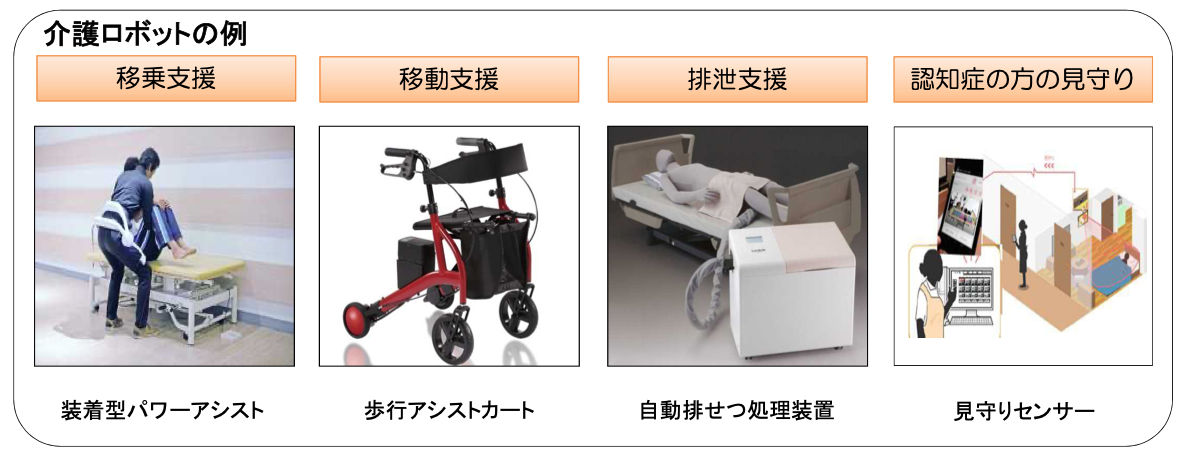
\includegraphics[scale=0.6]{figures/care_robots}
 \caption[介護ロボットの例]{介護ロボットの例 \label{care_robots}}
 \end{center}
\end{figure}

政府としても,介護ロボットを現場に導入することを支援しており,地域医療介護総合確保基金を始めとした各種助成金の設立やニーズ・シーズ連携協調のための協議会の設置を行っている.
第二に,ハイテク福祉機器とは新しい要素(アミューズメントやアート等)を取り入れたり、ICTやIoTといった技術を採用した福祉機器のことである.
ハイテク福祉機器の登場は,停滞気味であった福祉機器市場全体を押し上げる要因となるほどのインパクトを持っており,H.C.R.2018という国際フォーラムも開かれるほど注目を集めている.
具体的なプロダクトについて紹介する.図\ref{yubicommnnication}のように,有限会社オフィス結シェアの提供する指伝話コミュニケーションパックは,指伝話メモリで作成したコンテンツ集で,指伝話メモリのカードを選択してさまざまな機能を実現することができる.指伝話プラスや指伝話文字盤など他のアプリをホーム画面に戻らずに呼出,SMSやメールの送信,ウェブサイトやYouTubeを開く,iOSのショートカットを用いてiOSの機能を利用するといったことを行うための,実用的なサンプルセット集である.

\begin{figure}[htb]
 \begin{center}
 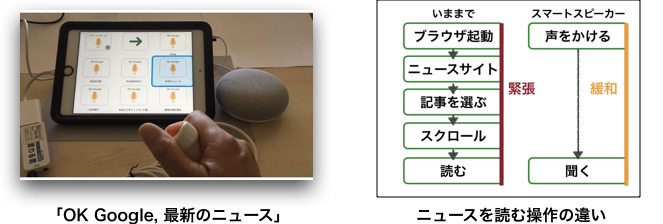
\includegraphics[scale=0.6]{figures/yubicommunication.png}
 \caption[コミュニケーションの例]{コミュニケーションの例 \label{yubicommnnication}}
 \end{center}
\end{figure}

会話が困難であったり,日常生活での移動が困難な要介護者への支援として各施設に導入され,介護士の負担軽減の一助となっている.

また,上記のような医療に関する技術は,高齢者自身の自立生活支援,高齢者介護の支援,生活の質(QOL)と快適性の高揚とその維持など,高齢者に対する生活支援分野においては,その使用者が被介護者か介護者により自立支援技術と介護支援技術に分けられる.\\
・自立支援技術 \\
排泄,入浴,調理,食事,就寝・起床,洗濯,清掃,義肢・装具,移乗,生活圏移動 \\
・介護支援技術 \\
排泄,入浴,清拭,褥瘡予防,食事,就寝・起床,移載・移動,監視 \\
また,これら技術には開発の優先順位が設けられている.以下の表\ref{tech_classiication}では,高齢者を自立意識が高い,低い,認知症の3パターンで分類したものと,被介護者の状態として全介護,半介護,身体異常の3パターンで分類したものとのマトリクスを示している.

\begin{table}[htb]
  \caption[介護技術の分類]{介護技術の分類}
  \label{tech_classification}
  \centering
  \begin{tabular}{r|c|c|c}
     & 全介護 & 半介護 & 身体異常 \\ \hline
    自立意識強い & 自立支援 & \quad & \quad \\
    自立意識弱い & \quad & \quad &  \quad \\
    認知症 & \quad & 介護支援 & \quad \\
    \end{tabular}
\end{table}

・自立支援 \\
自立意欲が高いにもかかわらず自立できていないことに対する支援機器が必要 \\
・介護支援 \\
一部介護を要する自立意欲の弱い高齢者には肉体的・精神的・時間的に大きな負担 \\
表\ref{tech_classification}にあるように,全介護の状態でありながらも,自立意識の高い被介護者と,半介護の状態でありながら,自立意識が弱かったり,認知症である場合に,それぞれ自立支援機器と介護支援機器の開発が必要とされる.

\subsection{医療技術導入における課題}

前述の支援機器の実用化には以下のように多くの問題点が存在する.

\begin{itemize}
 \item 性能不十分
 \item 操作複雑
 \item 寸法・重量
 \item 高価
 \item 危険
 \item 公害
 \item プライバシーの侵害
\end{itemize}

これら問題により,新技術の導入は医療サービス被提供者にとってはもちろん,医療機関にとって簡単に行うことができない.これら技術の導入が進んで来なかった背景として,そもそも技術として不完全であることに加え,現場の忙しい看護師や医師たちが簡単に使えるようなものでなければいけないことなど多くの制約があり,中でも,導入した際の効果検証ができないことが,意思決定の大きなボトルネックとなっている.また,病院は収益が順調に出ている状態だと,リスクをとって環境を改善するインセンティブが湧きづらく,こういった技術導入へのインセンティブが働かないことも大きな課題として挙げられる.

以上のように,最新技術の導入等の実験を行い,それらの効果検証が出来る医療シミュレータの開発が急を要しているものの,医療現場はプライベートな空間であり,これまで現実データを十分に獲得することが出来ず,有用なシミュレータの構築が難しかった.しかし,今後の日本における医療の重要性を考えると,個人の特性や意志を持った主体として介護者,被介護者を取り扱い,それらの詳細な相互作用を取り入れたシミュレータの構築が必要であると考えられる.

シミュレーションを行う際に気を付けなければならないのは,シミュレーションで用いる行動ルールのパラメータの妥当性とその客観性である.実際の介護の動きの計測結果から客観的に抽出されるルールやパラメータを入力とするシミュレーションが理想的である.しかし現在のところ,行動ルールのパラメータを抽出することを可能にするほどの精度の高い人流計測をするための研究はあまりされていない.これは一つには現在主流である単純な画像解析による手法の限界,もう一つには介護という環境がプライベートな空間であり,そもそも計測をできるような環境にない,という事が挙げられる.

\section{目的}

我が国日本では,医療技術の研究が盛んに行われているのにも関わらず,それらの導入・浸透には至っていない.そこで本論文では,各医療機関がそれら技術の導入の意思決定につながるシミュレーションモデルを構築することを目的とする.本研究の第一ステップとして,現在医療の現場で大きな課題となっている排泄介助にスコープを当て,排泄介助のシミュレーション上で技術の性能評価を行い,それによって技術の導入促進の意思決定に資するプラットフォームの構築をおこなう.

\section{本論文の構成}

1章では本論文の研究背景として,日本,医療界の諸課題について説明を行った.それに加えて課題の解決を目指す技術の紹介を行い,それらを導入する上での課題点を整理することで本論文の目的を示した.
2章では,提案手法についての説明をしている.3章では提案手法の数値実験により手法の検証を行う.4章では3章で得られた結果をまとめ,それらから得られる示唆についての考察を行い論文のまとめとする.
